\documentclass[../diploma.tex]{subfiles}
 
\begin{document}

	\label{sec:subject_area}

	\subsection{Обзор существующих решений}
   
	\label{subsec:existing_solutions}

	Существует множество работ, исследующих различные аспекты систем вопросов и ответов: 
	определение наилучшего ответа \cite{article:burel2012, article:tian2013, article:gkotsis2014}, 
	определение качества ответа \cite{article:agichtein2008, article:chua2013}, 
	выбор ответов к новым вопросам из уже существующих \cite{article:berger2000, article:surdeanu2008, article:jeon2006}, 
	определение качества вопроса \cite{article:agichtein2008, article:li2012}, 
	а также вероятности получения ответа на него \cite{article:agichtein2009}. 

	Тем не менее, в рамках темы данной работы стоит обратить внимание на исследования, касающиеся первого обозначенного аспекта: определения наилучшего ответа.
	Все статьи, фокусирующиеся на этой теме, имеют общую структуру: они извлекают различные признаки из текстов ответов, а также метаинформацию, 
	а затем используют некоторый бинарный классификатор, обученный на размеченных данных.

	Были подробно рассмотрены особенности следующих работ:

	\begin{itemize}
		\item
		В одной из первых работ \cite{article:tian2013}, анализирующих данную проблему в разрезе сайта StackOverflow, 
		использовался классификатор <<случайный лес>> по признакам трех типов:
		соответствующих содержанию ответа, измеряющих похожесть вопроса и ответа, а также использующих метаинформацию.
		Отдельное внимание авторы уделили признакам, сравнивающим текущий ответ с остальными: например, то, насколько он похож на остальные ответы.

		\item
		Также достаточно важна работа \cite{article:gkotsis2014}, в которой, во-первых, проведено масштабное исследование $21$ различного сайта системы StackExchange,
		а во-вторых, представлена так называемая идея дискретизации признаков: 
		процесс получения нового признака путем сортировки значений одного из старых и замены его значений на порядковый номер в получившемся списке 
		(эта идея будет раскрыта более подробно далее).
		Тем не менее, в рамках этой работы авторы никак не учитывают текст вопроса, 
		хотя это, безусловно, важная составляющая при определении правильности ответа на вопрос.

		\item
		Наконец, нужно упомянуть исследование \cite{article:burel2012}, проводившееся на наборах данных с трех сайтов системы StackExchange.
		Подход, представленный в работе, использует большое количество различных признаков, добиваясь наилучших результатов с помощью такой метаинформации, 
		как рейтинги ответа или пользователя, отвечавшего на вопрос, которые не использовались в нашей работе.
		Тем не менее, авторы предоставляют полученные метрики экспериментов для различных подмножеств признаков, 
		поэтому мы все равно можем сравнить полученные нами результаты с представленными в статье.
		В качестве классификатора авторы использовали чередующиеся решающие деревья \cite{article:freund1999}.
		Эта работа также не использует текстовые признаки вопроса.

    \end{itemize}

	Проанализировав имеющиеся исследования, можно отметить некоторые недостатки существующих решений:

	\begin{itemize}

		\item
		Несмотря на то, что во всех работах анализируется содержание текста ответа, в них никак не учитываются семантические значения слов, 
		а также порядок слов в предложении и их контекст, авторы используют лишь некую глобальную информацию, извлекаемую из текста.

		\item
		Некоторые работы также не используют специфику сайта StackOverflow, вопросы на котором написаны техническим языком и с достаточно большим количеством терминов, 
		а также могут содержать фрагменты исходного кода.

	\end{itemize}


    \subsection{Векторное представление текстов}

	\label{subsec:word_embedding}

    При работе с текстами в задачах обработки естественного языка требуется представлять слова и тексты в виде векторов, чтобы с ними было удобнее работать в дальнейшем. 
    Существует несколько подходов к векторному представлению текстов.

    
    \subsubsection{Bag of Words} 
    	
   	Bag of Words \cite{article:bag_of_words}~--- это одно из самых простых представлений, первые упоминания о котором датируются еще 1950-ми годами.

   	Основная идея состоит в том, что каждый документ представляется в виде вектора, размерность которого равна размеру словаря, 
   	а $i$-я компонента равна $1$, если $i$-ое слово из словаря присутствует в документе, и $0$~--- иначе.
   	При этом существуют различные модификации этого метода: могут не учитываться так называемые <<стоп-слова>>, 
   	которые встречаются слишком часто и не несут в себе никакой информации о содержании документа;
   	вместо бинарных значений компонент могут также использоваться количество вхождений слова в документ либо мера \texttt{TF-IDF} \cite{article:tf_idf}, 
   	когда значение $i$-й компоненты определяется по формуле: 
   	\begin{equation} 
   		\label{eq:tf-idf}
   		w_i = tf_i \cdot \log \frac{N}{df_i}
   	\end{equation}
   	где 
   	$tf_i$~--- количество вхождений слова в документ,
   	 
   	$N$~--- количество документов в корпусе данных, 

   	$df_i$~--- количество документов, в которых встречается данное слово.

   	Подобная модификация позволяет учитывать, насколько то или иное слово часто встречается в других документах: 
   	давать больший вес более редким и информативным словам и игнорировать шумовые слова.

   	Пример применения базового представления Bag of Words со стоп-словами можно видеть на рисунке \ref{fig:bag_of_words}.
   	\vskip 1em

   	\begin{minipage}{\linewidth}
   	    \centering
		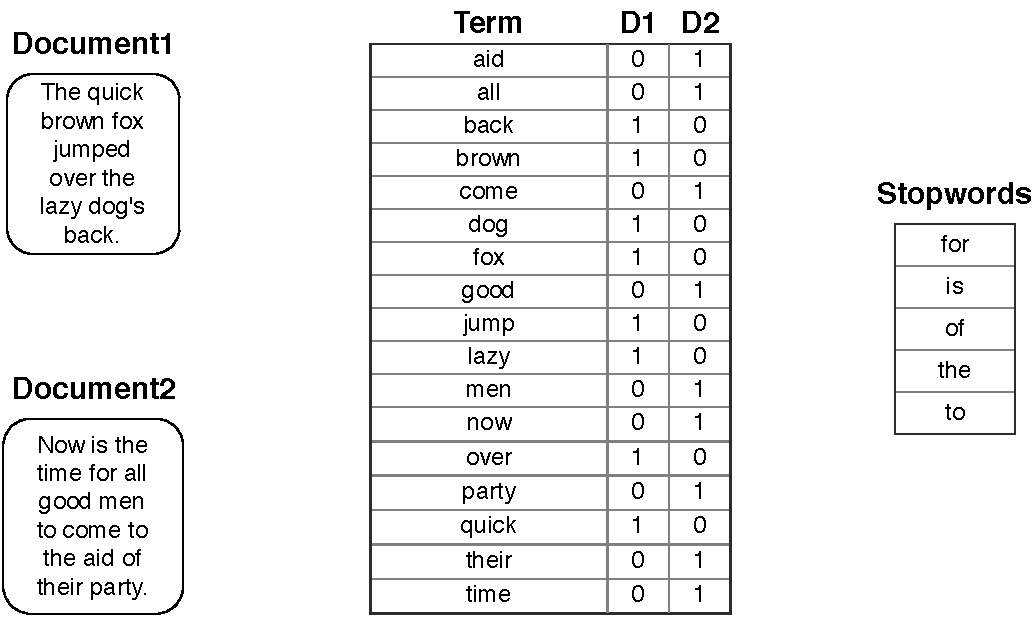
\includegraphics[width=0.9\linewidth]{images/bag_of_words.pdf}
   		\captionof{figure}{Пример работы представления Bag of Words}
		\label{fig:bag_of_words}
   	\end{minipage}
    	
	\subsubsection{Word2Vec} 

	Другой подход состоит в последовательной векторизации слов текста, а затем работе с этой последовательностью векторов.

	В $2013$ году был представлен Word2Vec \cite{article:word2vec}~--- способ векторизации слов, основанный на нейронных сетях.
	Основная идея метода состоит в предположении о том, что слова, находящиеся в похожих контекстах, 
	скорее всего будут значить похожие вещи, то есть будут семантически близкими.
	В данном случае под контекстом подразумевается набор слов из окна фиксированный ширины вокруг текущего слова.
	Тем не менее, этот контекст можно использовать для обучения двумя разными способами, поэтому в Word2Vec используется один из двух типов алгоритма:

	\begin{itemize}
		\item
		\textbf{Модель CBOW (Continuous Bag of Words)} (рисунок \ref{fig:cbow}). 

		В данной модели используется нейронная сеть с одним скрытым полносвязным слоем с функцией активации \texttt{ReLU} \cite{article:relu}.
		Обучение происходит следующим образом: корпус имеющихся текстов обрабатывается скользящим окном, выделяя контексты фиксированной ширины, 
		на вход сети подается контекст, представленный в виде вектора размерности длины словаря, полученный по модели Bag of Words, описанной ранее, 
		а на выходе ожидается вектор, в котором $i$-я компонента обозначает вероятность того, что в центре окна $i$-е слово.
		Для повышения производительности алгоритма используется негативное семплирование, 
		позволяющее вместо расчета всех возможных контекстов для функции потерь использовать фиксированное количество случайных контекстов.
		В качестве итогового векторного представления слов используется матрица весов скрытого слоя.

		Таким образом, мы пытаемся по данному контексту научиться предсказывать слово.
		
		\item
		\textbf{Модель Skip-gram} (рисунок \ref{fig:skip-gram}). 

		Альтернативой первой модели является модель Skip-gram.
		Она имеет схожую архитектуру, но при этом основывается на обратной идее: предсказании контекста по слову, 
		то есть получая на вход слово как единичный вектор, она пытается предсказать вероятности вхождения каждого из слов в контекст текущего.			
	\end{itemize}

    \vskip 1em
    \begin{figure}[ht]
        \begin{subfigure}{0.49\linewidth}
        	\centering
        	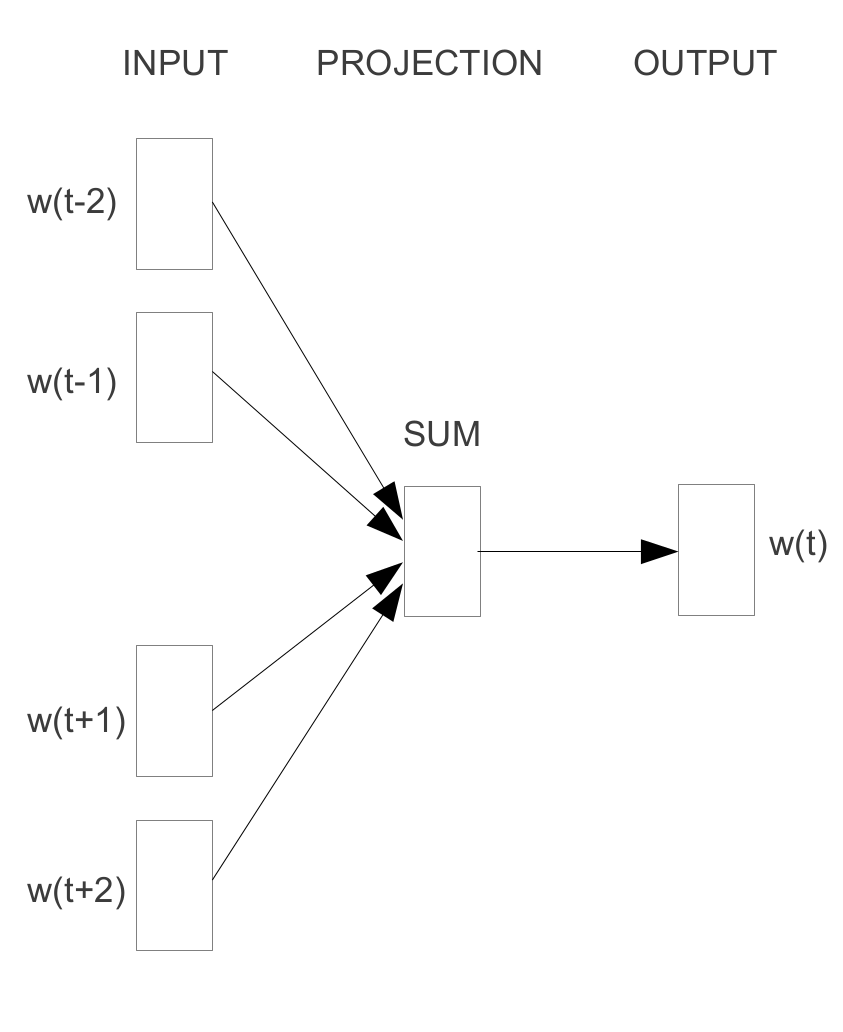
\includegraphics[width=\linewidth]{images/cbow.png}
        	\caption{\label{first}Архитектура модели CBOW}
        	\label{fig:cbow}
        \end{subfigure}
        \begin{subfigure}{0.49\linewidth}
        	\centering
        	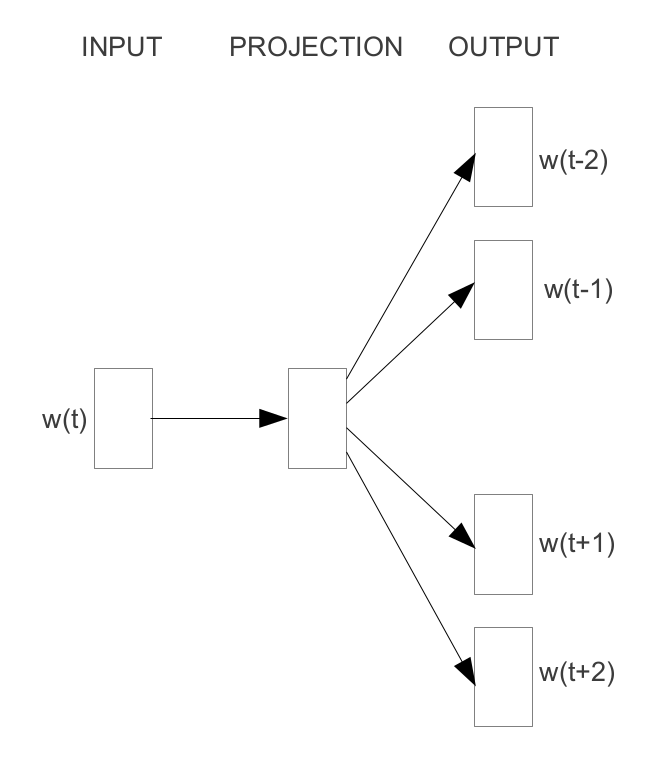
\includegraphics[width=\linewidth]{images/skip-gram.png}
        	\caption{\label{second}Архитектура модели Skip-gram}
        	\label{fig:skip-gram}
        \end{subfigure}
     	\caption{Модели Word2Vec}
    \end{figure}

    Стоит отметить, что для получения векторных представлений хорошего качества требуется обучение Word2Vec на большом корпусе неразмеченных текстов 
    (больше миллиарда слов).
    Интересной особенностью полученных векторизаций является не только близкое расположение векторов, отвечающих за близкие по смыслу слова, 
    но и сохранение семантических отношений между словами: 
    например, разность векторов, соответствующих словам <<король>> и <<королева>> очень близка к разности векторов <<мужчина>> и <<женщина>>.   

	\subsubsection{Fasttext}  

    У предыдущей модели есть один достаточно важный недостаток: 
    она не позволяет получать векторные представления слов, которые не встречались в обучающей выборке.
    
    Для решения этой проблемы используется модификация Word2Vec~--- Fasttext \cite{article:fasttext}.
    Если раньше в качестве представления слова мы использовали единичный вектор, 
    то в модели Fasttext из слова также выделяются все $n$-граммы~--- непрерывные подстроки длины $n$ (в базовой версии для всех $n$ от $3$ до $6$), 
    и в качестве представления слова берется взвешенная сумма векторов, соответствующих $n$-граммам.

    Подобный трюк позволяет получать векторизации для слова не из словаря, используя векторизации его $n$-грамм.

    \subsection{Нейронные сети}

    \label{subsec:neural_nets}

    За последние годы в области обработки естественных языков, в частности для задачи классификации текстов, нейронные сети стали показывать блестящие результаты.
    Ключевым эффектом является векторное представление целого текста, которое отражает его семантику, то есть смысл, заложенный в нем.

    Для этого используются две принципиально разные архитектуры, описания которых представлены ниже.

	\subsubsection{Рекуррентная нейронная сеть}

	Базовые идеи архитектуры рекурретных нейронных сетей (RNN~--- recurrent neural network), были разработаны еще в 1980-е годы.
	В основе этой архитектуры лежит использование рекуррентных слоев (рисунок \ref{fig:rnn_layer}), 
	позволяющих работать с данными, которые являются некоторой последовательностью.
	Для этого в качестве входных данных на каждую следующую ячейку RNN поступает не только новый элемент последовательности, 
	но и некоторая информация из состояния предыдущей ячейки.
	
	\vskip 1em               
    \begin{figure}[ht]
   	    \centering
		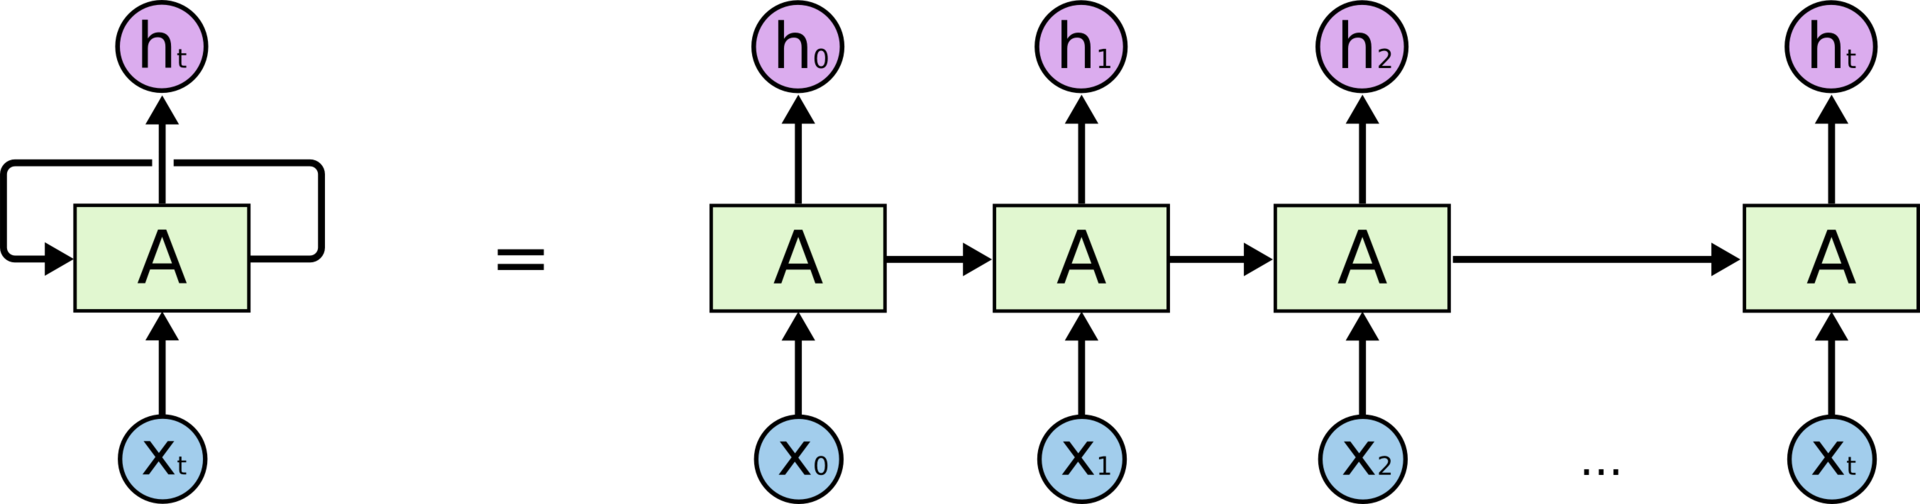
\includegraphics[width=0.9\linewidth]{images/rnn.png}
   		\captionof{figure}{Рекуррентная нейронная сеть}
		\label{fig:rnn_layer}
   	\end{figure}

   	Данный механизм может помочь и в решении задачи классификации текстов~--- последовательности слов, поскольку позволяет
    учитывать связь различных слов и предложений друг с другом. 
   	Для векторизации слов может быть использован один из методов из подраздела \ref{subsec:word_embedding}.

   	Тем не менее, в текстах часто важен достаточно широкий контекст, а обычные RNN на практике оказываются неспособны захватывать подобные связи
   	из-за проблемы затухающего градиента: при увеличении длины контекста норма градиента может экспоненциально убывать, 
   	из-за чего влияние текущего входа не может распространяться слишком далеко.
   	Чтобы избежать подобной проблемы, были придуманы \texttt{LSTM}-ячейки \cite{article:lstm} (рисунок \ref{fig:lstm}), 
   	которые способны сохранять информацию в течение длительного времени.

	\vskip 1em               
    \begin{figure}[ht]
   	    \centering
		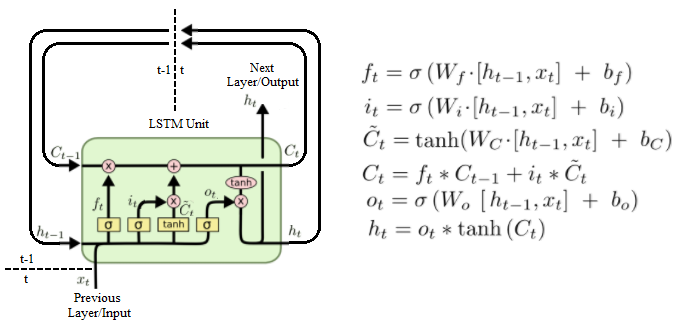
\includegraphics[width=0.9\linewidth]{images/lstm.png}
   		\captionof{figure}{\texttt{LSTM}-ячейка}
		\label{fig:lstm}
   	\end{figure}

   	Подобная архитектура позволяет захватывать контекст слева, хотя при анализе текста важен контекст, окружающий слово с обеих сторон.
   	Для этого придумана модификация обычного рекуррентного слоя~--- двунаправленный рекуррентный слой \cite{article:bi_rnn}, 
   	который представляет из себя два слоя, в один из которых данные подаются на вход в прямом порядке, а в другой~--- в обратном, 
   	а в качестве выхода используется конкатенация выходов с этих двух слоев.

	\subsubsection{Сверточная нейронная сеть}

	Основой для сверточных нейронных сетей \cite{article:cnn} (CNN~--- convolutional neural network) служат сверточные слои, которые работают следующим образом: 
	на вход этому слою подается тензор, 
	после чего каждый фрагмент этого тензора скалярно умножается на ядро свертки, и получившийся тензор передается следующему слою сети.

	Несмотря на то, что изначально этот механизм применялся для работы с изображениями, 
	исследования последних лет \cite{article:text_cnn} показали, что он также эффективен и при работе с текстом.

	На рисунке \ref{fig:cnn} показан пример архитектуры, используемой для классификации текстов.
	В качестве входной матрицы подаются векторизованные представления слов текста, после чего к ним применяется свертка размером $k \cdot D$, 
	где $D$ --- размерность векторного представления, а $k$ --- параметр сети.
	Обычно используется несколько сверток с различными ядрами, при этом используются $k$, равные $2, 3, 5, 7$, что позволяет захватить контекст вокруг слова.
	После сверточного слоя используется глобальный \texttt{Max-Pooling} слой, который оставляет максимальное значение из каждой свертки, 
	тем самым позволяя уменьшить размерность данных.
	Получившиеся значения конкатенируются и отдаются на вход следующему слою.
	В данной архитектуре используется обычный полносвязный слой, с помощью которого определяется принадлежность текста к одному из двух классов.

	\vskip 1em               
    \begin{figure}[ht]
   	    \centering
		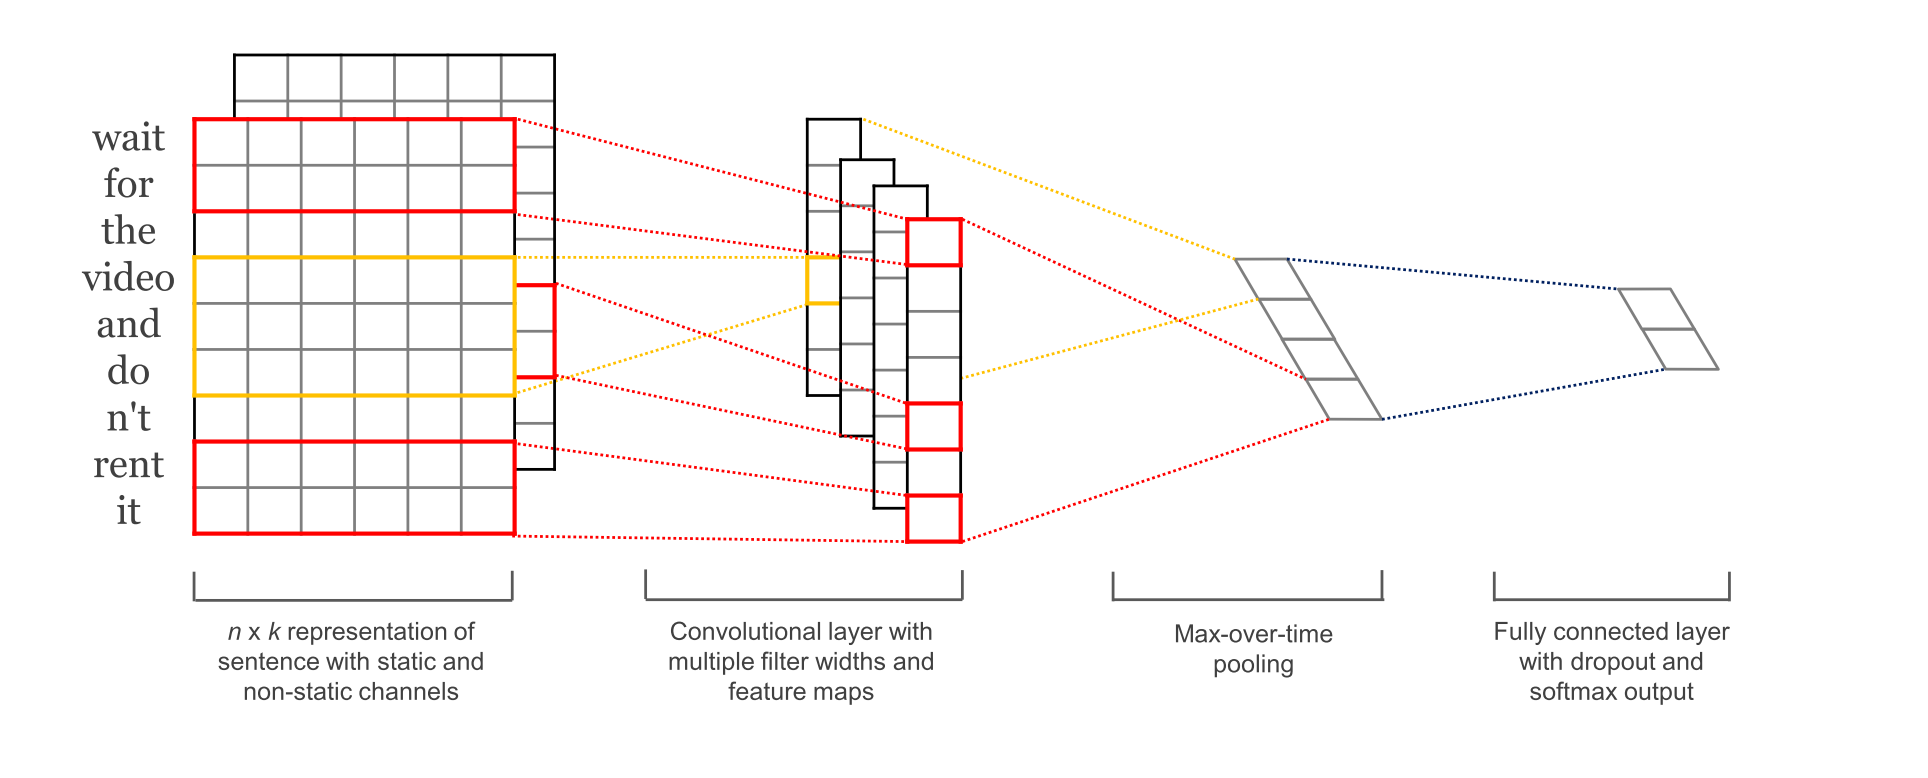
\includegraphics[width=1.1\linewidth]{images/cnn.png}
   		\captionof{figure}{Сверточная нейронная сеть для классификации текстов}
		\label{fig:cnn}
   	\end{figure}



\end{document}

